%
% File acl2017.tex
%
%% Based on the style files for ACL-2015, with some improvements
%%  taken from the NAACL-2016 style
%% Based on the style files for ACL-2014, which were, in turn,
%% based on ACL-2013, ACL-2012, ACL-2011, ACL-2010, ACL-IJCNLP-2009,
%% EACL-2009, IJCNLP-2008...
%% Based on the style files for EACL 2006 by 
%%e.agirre@ehu.es or Sergi.Balari@uab.es
%% and that of ACL 08 by Joakim Nivre and Noah Smith

\documentclass[11pt,a4paper]{article}
\usepackage[hyperref]{acl2017}
\usepackage{times}
\usepackage{latexsym}

\usepackage{url}

\aclfinalcopy % Uncomment this line for the final submission
%\def\aclpaperid{***} %  Enter the acl Paper ID here

%\setlength\titlebox{5cm}
% You can expand the titlebox if you need extra space
% to show all the authors. Please do not make the titlebox
% smaller than 5cm (the original size); we will check this
% in the camera-ready version and ask you to change it back.

% added
\usepackage{graphicx}
\usepackage{amsmath}
\usepackage{dsfont} %to have \mathds{1}

\newcommand\BibTeX{B{\sc ib}\TeX}

\title{Identification and quantification of colours in children's drawings}

\author{Christelle Cocco ${}^1$, Rapha\"el Cer\'e ${}^2$, Aris Xanthos, ${}^3$  Pierre-Yves Brandt ${}^1$\\
  ${}^1$Institute for Social Sciences of Religions / University of Lausanne, Switzerland \\
  ${}^2$Department of Geography and Sustainability / University of Lausanne, Switzerland \\
  ${}^3$Department of Language and Information Sciences / University of Lausanne, Switzerland \\
  {\tt \{Christelle.Cocco, Raphael.Cere, Aris.Xanthos, Pierre-Yves.Brandt\}@unil.ch} \\
%  \And
%  Second Author \\
%  Affiliation / Address line 1 \\
%  Affiliation / Address line 2 \\
%  Affiliation / Address line 3 \\
%  {\tt email@domain} \\
  }


\date{}
\begin{document}
\maketitle
\begin{abstract}
[TO UPDATE AT THE END] Children's drawings reveal that developing colour retrieval technics
must consider various aspects of what is a colour from the flow of
energy (for physics) to discrete information (for humantities and human
sciences). Hence, the proposed method deals with color variety measures
and colours quantifications upon the drawing to respond at specific
queries e.g. ``Which colours appear?'', or ``How much yellow appears?''.
\end{abstract}


\section{Introduction}\label{introduction}

In computer vision, there are well developed techniques to analyse and retrieve natural images (e.g.~pictures or videos). 
However, the status of the image in humanities or in human sciences depends more on the perception of the image. Moreover, the images are not necessarily natural (e.g.~paintings or drawings). Therefore, specific techniques need to be developed according to precise research questions of humanities.

For the multicultural and interdisciplinary project: ``Drawings of gods''\footnote{This project is supported by the Swiss National Science Foundation (SNSF), grant number: CR11\textbar1\_156383.}, whose the main fields are developmental psychology and psychology of religion, children's drawings of gods were collected in several countries \cite[for more details about this project, see \textit{e.g.}][]{BrandtKagataSpittelerGillieronPaleologue2009,Dandarova2013,DandarovaRobertDessartSerbaevaEtAl2016}.\footnote{The database of the project is available on \url{http://ddd.unil.ch/}.} 
In order to analyse these drawings, it would be helpful to identify and quantify the colours used by the children in their drawings. 
Indeed, several research questions in the project are related to colours, such as ``Which colours are used to draw god?'', ``Are the same colours utilised in all countries?'', ``Did older children use more or less colours than younger ones?''

To answer these questions, the first step is to define a set of colours. 
However, although it is possible, with a computer, to obtain precise values defining the colour of a pixel, there is no universal colour set.
It is even difficult to align the perception of two humans.
Indeed, The human colour perception occurs through the radiance incident upon
the retina on which three photoreceptor cells, named cones, are located.
Only these three photoreceptors are necessary, corresponding to the
\emph{Red}, \emph{Green} and \emph{Blue} numerical components (RGB) of
the pixel
\(\vec{s} = \{ s^{\tt \scriptstyle R}, s^{\tt \scriptstyle G}, s^{\tt \scriptstyle B} \}\),
to describe a colour using appropriate spectral functions. Standard
curves have been adopted in 1931 by the Commission International de
l'Eclairage (CIE) to specify the colour by those three numbers from
spectral power distribution transformation.

Although the CIE standard exists, only computers are able to assign
those three numbers to a colour in a precise manner. Therefore, any
human assignment is basically obsolete due to the influence of an
individual's interpretation of the colour (e.g. ``Where can I put a
threshold between red and orange?'', ``Is it not already brown?'').
Moreover, the human perception of colour distribution of an image can be
drastically different in terms of vision \cite{jobson1997} and,
respectively, in terms of perception depending on the context e.g.
\emph{Chubb illusion} or \emph{Checker shadow illusion}.


MORE DIFFICULT... children's drawings
dataset. The particularity of this kind of image depends on the drawer's
colour choices. It can be intentional according to his/her own
perception and his/her human singularity or constraints according to
colour availability. Subsequently, the resulting object analysis is
technically constrained: the final colours are altered by the
digitalisation encoding, as well as the quantification of colours.









While colours can be precisely defined in computation, human categories
are more conceptual, as explained by \citet{wittgenstein1977}:

\begin{quote}
	``When we're asked about''What do the words `red', `blue', `black',
	`white', mean?" we can, of course, immediately point to things which
	have these colours, - but our ability to explain the meanings of these
	words goes no further! For the rest, we have either no idea at all of
	their use, or a very rough and to some extent false one." (68,I)
\end{quote}

Perception according to
\cite[][p. 35 and p.87]{pastoureau2017}: complex phenomenon,
neurobiology and cultural. Perception depends on the age and on the
society. It is not a universal law. West perception not equal to world
perception.


As explained in the
introduction, the second aim of this paper is to fill the gap between
the universal human categories and the exact colour of each pixel.
However, it is difficult or even impossible to define universal human
categories. Some attempt in psychology\ldots{} {[}VOIR TRAVAUX D'ANNA
FRANKLIN{]} Various languages implies various names for the
colours\ldots{} According to the historian and colour specialist,
Pastoureau, a colour is not equivalent to the shade of a colour, which
has neither its own history, nor its own symbolic, unlike colours
\cite[][p. 12 and p. 63]{pastoureau2017}. Thus, he counts 11 colours for
the West {[}VERIFIER{]}, whose 6 from the first rank: white, red, black, green, yellow and blue; and 5 from the second rank: pink, orange, purple (violet), gray and brown.

He also explains that colours are mental categories
\cite[][p. 36]{pastoureau2017} and he differentiates colours according
to physical laws (spectral colours, Newton) and colours which are the
base of our vocabulary based on the classification of Aristotle
\cite[][p. 90-91]{pastoureau2017}.

Thus, it is impossible to obtain universal categories of colours and
there is a ``big'' gap between spectral colours and human categories of
colours\ldots{}.

In order to attest these categories, we asked to
\ldots{} human annotators (two Russians, one Swiss/Iranian, one/two
Swiss people, one Belgian), to write the colour names of the colour of a
set of\ldots{} drawings. In the second phase, annotators had to select
presence or absence of colours in a list based on the Munsell system for
another set of drawings (\ldots{} were part of both sets). Moreover,
they had space to write name of missing colours.
Kappa...... [CITER POUR POOLED KAPPA]

For human sciences questions, it is necessary to develop specific
techniques, since the aim is not to precisely find the nuance of the
colour in the drawing, but to determine the diversity of colours on the
one hand (gap 1) ; and to figure whether there is one colour that stands
out from a set of colours on the other hand (gap 2).

 Regarding the definition of a set of
colours -\textgreater{} Berlin and Kay and so on\ldots{}. {[}to be
completed{]}

Indeed, two aspects of the quantification of a drawing's colours are
developed:

\begin{enumerate}
	\item
	the gap between the human perception (continuous colours) and the
	colour categorisation (discrete colours)
	\cite[see e.g.][]{parragaakbarinia2016, benavente2008, berlinkay1969}, [PERCEPTION]
	\item
	the gap between the human categories of colours (ideally universal)
	and the exact colour of each pixel in the image (continuous colours)
	\cite{khan2012, khan2013} [STATE OF THE ART?]
\end{enumerate}

\section{State of the art}

A number of previous researches in computer vision proposed promising
descriptors such as colour histograms \cite{sun2006} or colour names
\cite{weijer2009, lindner2013} through mapping learned from images.
However, their aims differed from the one found in the human sciences
and described above. For instance, when colour is used in image
retrieval, the aim is to find which images of a dataset correspond to
the one stated as the query. Thus, the main point is to determine if the
colours of the query and those of the dataset are similar, no matter
which colour it is. More specifically, the paper of
\cite{konyushkova2015} proposes a solution closer to the aim of finding
the set of colours displayed in children's drawings with the well-known
method of \emph{K-means}. However, it allows to extract mean colours for
a set of drawings which is not the aim here.

Most of the researches about colours in
computer vision concern the field of image retrieval. In this type of
researches, the aim is to find if two images have the same colours and
not, as in this project, to discover if the pixels in the image belongs
to a certain colour of a set {[}REF{]}.

When the aim is still to find colour groups, the
K-means algorithm is often used \cite[see e.g.][]{yendrikhovskij2001,konyushkova2015,hulee2007}. However, there are two main
drawbacks with this method: 1) it is necessary to define the number of
clusters (K), thus the number of colours a priori; 2) for each cluster,
we can obtain a mean of colours belonging to this cluster and these
means can be difficult to name and to distinguish.

Possible with the Munsell colour space, as done by \citet{kimbaelee2007}, near human perception, but no linear transformation between
RGB and Munsell \cite[see e.g.][]{zhangsokhansanjwuetal1998}

\section{Methods}\label{methods}
{[}SUITE A REECRIRE{]} Therefore, we decided to start with a set of
colours. At this point, there are two main choices to make: 1) chose the
colour space and 2) definition a set of colours.

{[}SUITE A REECRIRE{]} Concerning the first choice, there are many
colours spaces \cite{tkalcictasic2003}, but RGB can be stated as ``the basic colour space''. For instance, Gong et al.~1998
for their image indexing and retrieval method based on the NBS colour
distance, use the HVC space.

\begin{itemize}
	
	\item
	First tests: HSV with range of colours -\textgreater{} difficult to
	define the limit between two colours
	\item
	Final choice: distance to colours
	
	\begin{itemize}
		\item
		Final choice: RGB with a set of colours, each from light to dark and
		distance to this colour
	\end{itemize}
\end{itemize}



\subsection{Data}

N = 1212 children's drawings of gods, drawing
$k = 1,\dots, N$, which are mainly studied from the psychology of
religion perspective \cite[see][]{ddds}. 

\subsection{Preprocessing}
Each image $S = (\vec{s}_{ij})$ contains $i \times j$
pixels ($\vec{s}$) and each pixel has three values (for Red, Green and Blue), \textit{i.e.}
$\vec{s} = \{ s^{\tt \scriptstyle R}, s^{\tt \scriptstyle G}, s^{\tt \scriptstyle B} \}$.

As a first step, each image $k$ is resized with the imresize
module of the scipy.misc package, in such a way that the longer side is
equal to 320 pixels. Note here that the drawings are
rescaled at the same scale but not precisely at the same size.


\subsection{Identification of colours}

% \hypertarget{from-colour-categories-to-exact-colour-of-pixels}{%
% \subsection{From colour categories to exact colour of
% pixels}\label{from-colour-categories-to-exact-colour-of-pixels}}




In order to fill the second gap between the categories of colour and its
perception, a method based on the image in the RGB colour space is
proposed. With a similar approach of the one developed by
\cite{kimbaelee2007} in the the Munsell colour system, the dissimilarity
between each pixel and a set of colours is computed. More precisely, for
each image, a squared Euclidean dissimilarity is computed between each
pixel \(\vec{s}\) and a set of $L = 117$ colours (see Figure~\ref{colour_set}) defined in RGB:
\(\vec{c_l} = \{ c^{\tt \scriptstyle R}_{l}, c^{\tt \scriptstyle G}_{l}, s^{\tt \scriptstyle B}_{l} \}\),
with $l = 1, ..., L$.

\begin{figure}
	\centering
	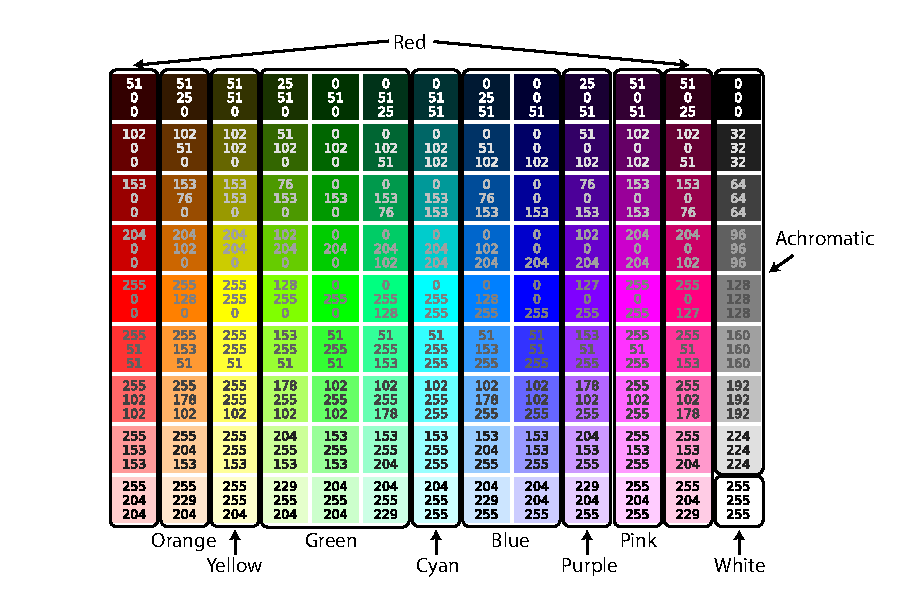
\includegraphics[width=0.5\textwidth]{figures/Col_tab.pdf}
	\caption{Set of 117 colours aggregated in 10 groups. \label{colour_set}}
\end{figure}

Then, for each pixel \(\vec{s}\), the less dissimilar \(c_l\) is considered as
the colour of the pixel:
\begin{equation*}
c(\vec{s}_{ij}) := \operatornamewithlimits{argmin}_{l \in [1,L]} \| s_{ij} - c_{l} \|^{2}
\end{equation*}

Finally, according to the Figure~\ref{colour_set}, the 117 colours are grouped into $G = 10$
main colours ($g = 1, \dots, G$), \textit{i.e.} red, orange, yellow, green, cyan, blue, purple, pink,
white and achromatic. Therefore, each pixel belongs to one of these
10 groups and the name of the colour of each pixel is defined as $C(\vec{s}_{ij}) = \mathds{1}(c(\vec{s}_{ij}) \in g)$ [CE N'EST PAS ENCORE CA, MAIS ON S'EN APPROCHE, ON NE VEUT PAS 1, MAIS LE NOM... $= g \quad \textrm{if} \quad c(\vec{s}_{ij}) \in g$ ?]. \footnote{Here and in the sequel, $\mathds{1}(A)$ denotes the \textit{indicator function} of event $A$, taking on the value 1 if $A$ is true, and 0 otherwise.}

For each drawing $k$, this permits us to obtain one
boolean matrix per colour $g$:
\begin{equation}
B^{g} = (b_{ij}^{g}) \quad \textrm{with} \quad b_{ij}^{g} =  \mathds{1}(C(\vec{s}_{ij}) = g)
\end{equation}

Thus, the number of pixels of each main colour $g$ for one drawing is defined as:
\begin{equation}
	f^{g} = \sum_{ij}b_{ij}^{g}
\end{equation}




{[}A COMPLETER + METTRE EXEMPLE{]}Then we can extract the proportion of
each colour used in each drawing (see table \ref{colquant}), as well as
the presence or absence of each colour. Thus, we can answer the
psychological research questions mentioned above. These methods are
applicable to other data and research, e.g.~studying the main colours
used by a painter according to various periods of his/her life.





[MET-ON LE CODE SUR GITHUB??? ET ENSUITE UN LIEN?]


\subsection{Colour diversity [ARIS]}


As a second step, in order to
count the number of colours used per drawing and to reduce the noise due
to the scan quality, a median filter of a \(3 \times 3\) is applied on
each boolean colour matrix $B^{g}$ and new matrices are obtained, namely
$B^{\prime g}$.

% \hypertarget{from-human-perception-to-colour-categorisation}{%
% \subsection{From human perception to colour
% categorisation}\label{from-human-perception-to-colour-categorisation}}

Concerning the first gap, through the \emph{state-of-art} of colour
retrieval, the most fruitful quantitative approach to translate color
choices between humans (drawer \(\leftrightarrow\) observer) is the
average amount of information provided by a stochastic source of colors
(the drawing) called the Shannon information entropy from the
information theory (Claude Shannon 1948).

To calculate the entropy, the common approach is first to convert the
drawing RGB color space into a greyscale using a linear-light conversion
where \(\vec{s}\) becomes a univariate measure \(s^{\tt \tiny CRT}\)

\[s^{\tt \scriptstyle CRT} = 0.2125s^{\tt \scriptstyle R} + 0.7154 s^{\tt \scriptstyle G}+ 0.0721 s^{\tt \scriptstyle B}\]

which reveals the intensity of light \cite{poynton1997}. This conversion
is only effective if the drawing is regarded solely as an optical record
of light intensity than the visual experience where other methods have
to be considered (see \cite{amy2005}).

For each \(i\) drawing a biased color distribution is considered to take
into account an certain user choice (such as a biased dice,
non-completely random). Consequently, we postulate that drawings are
independent to each other; singular in view of color used. The \(m\)
categories of grey for each drawing is measured by counting the \(j\)
number of \(S^{\tt \scriptstyle CRT}_m\) distinct pixel grey,
\(j = 1, \dots, m\) modalities. By construction, the relative
frequencies or proportions \(f_j = S^{\tt \scriptstyle CRT}_j/S\)
respect

\[S_j \geq 0 \qquad \sum_{j=1}^{m} S_j = S \qquad f_j = \frac{S_j}{S} \qquad \sum_{j=1}^{m} f_j = 1\]

The notion of variety of grey naturally seems to be a good value to
depict qualitatively the colors. The relative variety
\(\delta^{\tt \scriptstyle CRT}\) depends on the \(f\) proportion
observed. The number of each unique level of grey which appear
effectively in \(S^{\tt \scriptstyle CRT}\) is considered, \(f_j>0\)
thus \(\delta^{\tt \scriptstyle CRT} = m\).

However, \(\delta\) doesn't take into account the grey category
proportions. Because of Shannon, the entropy
\(H(S^{\tt \scriptstyle CRT})\) is a measure of the variety which yields
a quantity of the finesse (similar to the variance) of the
categorisation of the greyscale in \(m\) distinct grays.

\[ H(S^{\tt \scriptstyle CRT}) \equiv H(f) = -\sum_{j=1}^{m} f_j \log f_j \]

where
\(\log(s^{\tt \scriptstyle CRT}) \equiv \log_a(s^{\tt \scriptstyle CRT})\)
is the logarithmic function of \(s^{\tt \scriptstyle CRT} > 0\) into a
certain base \(a > 1\). Depend of the \(f\) distribution, the prevision
of \(s^{\tt \scriptstyle CRT}\) will be more of less uncertain. The
natural base used here is \(a = e\) then the entropy unit is in
\emph{nats} and \(0 \leq H(f) \leq log(m)\). The interpretation of this
quantity is: the higher the entropy value the larger the distribution
dispersion is. Figure \ref{entscatter}.

The so called perplexity is the exponential of the entropy in base
\(a\), \(M(f) = a^{H(f)}\), which yields a measure of the number of
effective categories in the uniform distribution of the same \(H(f)\)
and satisfies \(1 \leq M(f) \leq m\). Figure \ref{perpscatter}.

The weighted mean intensity {[}A CALCULER{]}.

Relation between entropy and perplexity via Gini \(G\) coefficient and
Lorenz courb Figure \ref{giniloenscatter}.

Those three quantities provide fundamental quantitative information
about human colour perception based on the pixel intensity: the higher
the entropy value the lighter the colour of the drawing, otherwise
coloured drawing, whereas the higher the number of types the coloured
drawing (see figure \ref{enttypesscatter}) and the higher the mean
intensity the lighter the drawing.



\section{Results [RAPHAEL]}

\subsection{Colour identification}

% \begin{table}
% \begin{tabular}[]{@{}cc@{}}

% \includegraphics[height=0.12\textwidth]{../img/jp04_to_m_rnx_08_07_nrx-r.jpg}
% &
% \includegraphics[width=0.22\textwidth]{../img/jp04_to_m_rnx_08_07_nrx-r.png}\tabularnewline
% \bottomrule
% \end{tabular}
% \caption{Colours quantification from the left image.} 
% \label{colquant}
% \end{table}

{[METTRE DES FIGURES D'UN EXEMPLE QUI FONCTIONNE ET D'UN AUTRE QUI NE FONCTIONNE PAS]}

\subsection{Colour diversity}

% \begin{figure}
% \centering
% \includegraphics[width=0.45\textwidth]{../../dev/entropy-mod-comhum.png}
% \caption{Entropy and effective categories logarithmic scatter plot.
% \label{entscatter}}
% \end{figure}

% \begin{figure}
% \centering
% \includegraphics[width=0.45\textwidth]{../../dev/perplexity-mod-comhum.png}
% \caption{Perplexity and effective categories logarithmic scatter plot.
% \label{perpscatter}}
% \end{figure}

% \begin{figure}
% \centering
% \includegraphics[width=0.45\textwidth]{../../dev/ginilorenz.png}
% \caption{\(G\) Gini coefficient with the associated Lorentz curve.
% \label{giniloenscatter}}
% \end{figure}

coucou
\begin{table}
	\begin{tabular}[!h]{cccc}
		
		\small Index &
		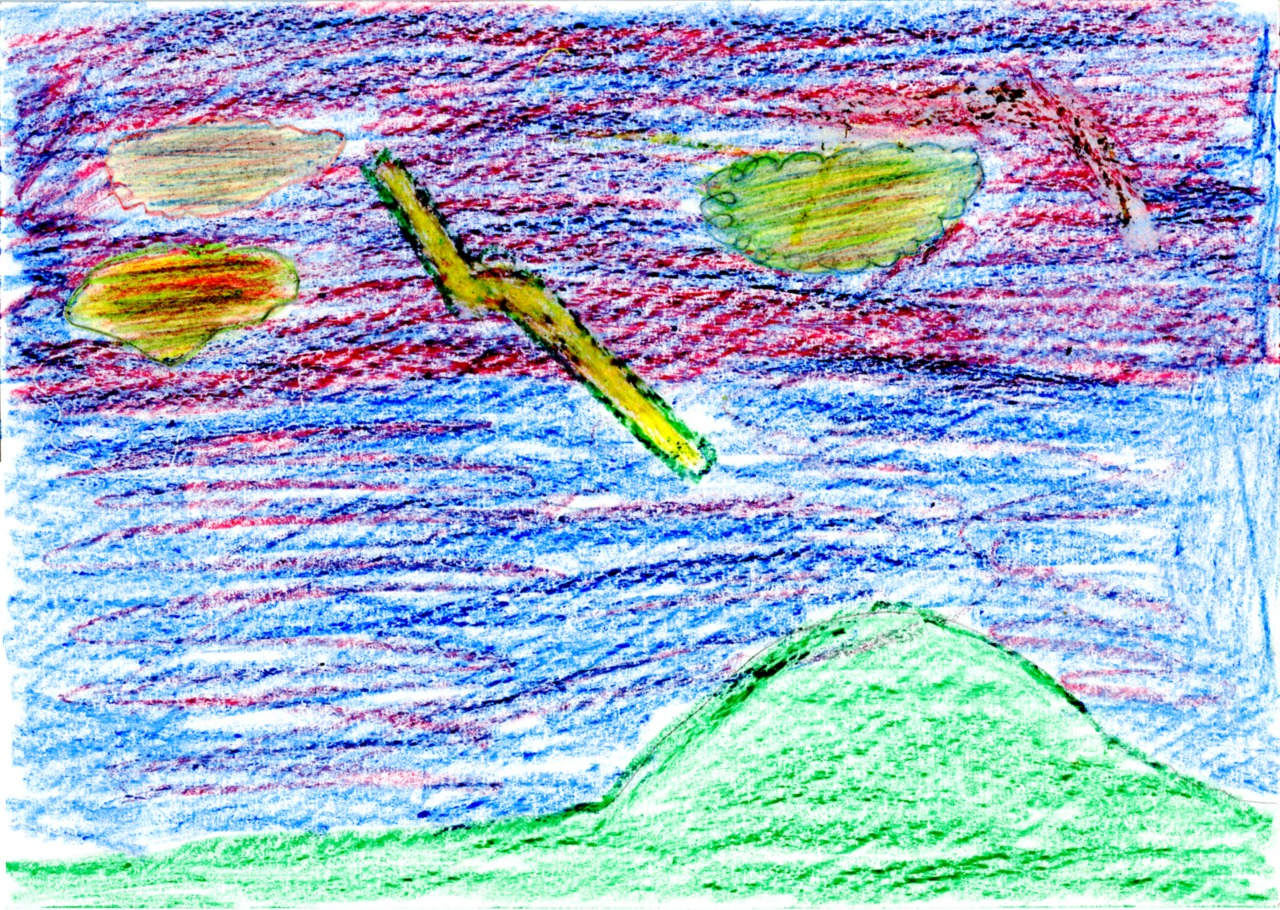
\includegraphics[height=0.06\textwidth]{figures/ru09_sp_m_rf_14_03_ale-r.jpg}
		& essai & essai \\
		% &
		% \includegraphics[height=0.06\textwidth]{../../DATA/IMAGE/jp04_fa_m_pkx_11_05_tyx-r.jpg}
		% &
		% \includegraphics[height=0.06\textwidth]{../../DATA/IMAGE/ch16_fr_m_rec_14_08_sim-r.jpg}\tabularnewline
		
		
		\small \(\mu^{\tt \scriptstyle CRT}\) & \small 0.696 & \small 0.876 &
		\small 0.999\tabularnewline
		\small \(\delta^{\tt \scriptstyle CRT}\) & \small 457068 & \small 37982
		& \small 41\tabularnewline
		\small \(H(S^{\tt \scriptstyle CRT})\) & \small 1.538 & \small 1.903 &
		\small 5.200\tabularnewline
		
	\end{tabular}
	\caption{Illustration of variety measures {[}METTRE A JOUR{]}. }
	\label{varietyill}
\end{table}

\section{Conclusion}

As a next step, since humans are more sensitive to colour patches than
to isolated pixels, a filter should be applied at the beginning of the
process, such as the Mumford-Shah Regulariser proposed by
\citet{erdem2009}. Indeed, when children (or adults) fill in an area of
the sheet with colour, the application is not regular and consequently
not all pixels of the zone are coloured. Thus, in order to avoid
underestimating the proportion of one particular colour, standardizing
colours by zone could help work around the possible issue.

\bibliography{bibliography}
\bibliographystyle{acl_natbib}

\end{document}
